\def\year{2020}\relax
%File: formatting-instruction.tex
\documentclass[letterpaper]{article} % DO NOT CHANGE THIS
\usepackage{aaai20}  % DO NOT CHANGE THIS
\usepackage{times}  % DO NOT CHANGE THIS
\usepackage{helvet} % DO NOT CHANGE THIS
\usepackage{courier}  % DO NOT CHANGE THIS
\usepackage[hyphens]{url}  % DO NOT CHANGE THIS
\usepackage{graphicx} % DO NOT CHANGE THIS
\urlstyle{rm} % DO NOT CHANGE THIS
\def\UrlFont{\rm}  % DO NOT CHANGE THIS
\usepackage{graphicx}  % DO NOT CHANGE THIS
\frenchspacing  % DO NOT CHANGE THIS
\setlength{\pdfpagewidth}{8.5in}  % DO NOT CHANGE THIS
\setlength{\pdfpageheight}{11in}  % DO NOT CHANGE THIS
%\nocopyright
%PDF Info Is REQUIRED.
% For /Author, add all authors within the parentheses, separated by commas. No accents or commands.
% For /Title, add Title in Mixed Case. No accents or commands. Retain the parentheses.
 \pdfinfo{
/Title (AAAI Press Formatting Instructions for Authors Using LaTeX -- A Guide)
/Author (AAAI Press Staff, Pater Patel Schneider, Sunil Issar, J. Scott Penberthy, George Ferguson, Hans Guesgen)
} %Leave this	
% /Title ()
% Put your actual complete title (no codes, scripts, shortcuts, or LaTeX commands) within the parentheses in mixed case
% Leave the space between \Title and the beginning parenthesis alone
% /Author ()
% Put your actual complete list of authors (no codes, scripts, shortcuts, or LaTeX commands) within the parentheses in mixed case. 
% Each author should be only by a comma. If the name contains accents, remove them. If there are any LaTeX commands, 
% remove them. 

% DISALLOWED PACKAGES
% \usepackage{authblk} -- This package is specifically forbidden
% \usepackage{balance} -- This package is specifically forbidden
% \usepackage{caption} -- This package is specifically forbidden
% \usepackage{color (if used in text)
% \usepackage{CJK} -- This package is specifically forbidden
% \usepackage{float} -- This package is specifically forbidden
% \usepackage{flushend} -- This package is specifically forbidden
% \usepackage{fontenc} -- This package is specifically forbidden
% \usepackage{fullpage} -- This package is specifically forbidden
% \usepackage{geometry} -- This package is specifically forbidden
% \usepackage{grffile} -- This package is specifically forbidden
% \usepackage{hyperref} -- This package is specifically forbidden
% \usepackage{navigator} -- This package is specifically forbidden
% (or any other package that embeds links such as navigator or hyperref)
% \indentfirst} -- This package is specifically forbidden
% \layout} -- This package is specifically forbidden
% \multicol} -- This package is specifically forbidden
% \nameref} -- This package is specifically forbidden
% \natbib} -- This package is specifically forbidden -- use the following workaround:
% \usepackage{savetrees} -- This package is specifically forbidden
% \usepackage{setspace} -- This package is specifically forbidden
% \usepackage{stfloats} -- This package is specifically forbidden
% \usepackage{tabu} -- This package is specifically forbidden
% \usepackage{titlesec} -- This package is specifically forbidden
% \usepackage{tocbibind} -- This package is specifically forbidden
% \usepackage{ulem} -- This package is specifically forbidden
% \usepackage{wrapfig} -- This package is specifically forbidden
% DISALLOWED COMMANDS
% \nocopyright -- Your paper will not be published if you use this command
% \addtolength -- This command may not be used
% \balance -- This command may not be used
% \baselinestretch -- Your paper will not be published if you use this command
% \clearpage -- No page breaks of any kind may be used for the final version of your paper
% \columnsep -- This command may not be used
% \newpage -- No page breaks of any kind may be used for the final version of your paper
% \pagebreak -- No page breaks of any kind may be used for the final version of your paperr
% \pagestyle -- This command may not be used
% \tiny -- This is not an acceptable font size.
% \vspace{- -- No negative value may be used in proximity of a caption, figure, table, section, subsection, subsubsection, or reference
% \vskip{- -- No negative value may be used to alter spacing above or below a caption, figure, table, section, subsection, subsubsection, or reference

\setcounter{secnumdepth}{0} %May be changed to 1 or 2 if section numbers are desired.

% The file aaai20.sty is the style file for AAAI Press 
% proceedings, working notes, and technical reports.
%
\setlength\titlebox{2.5in} % If your paper contains an overfull \vbox too high warning at the beginning of the document, use this
% command to correct it. You may not alter the value below 2.5 in
\title{Sokoban: PDDL Domain planning with Single-Agent}
%Your title must be in mixed case, not sentence case. 
% That means all verbs (including short verbs like be, is, using,and go), 
% nouns, adverbs, adjectives should be capitalized, including both words in hyphenated terms, while
% articles, conjunctions, and prepositions are lower case unless they
% directly follow a colon or long dash
\author{Written by Bachelor students from King's Collage London\textsuperscript \\  \\  % All authors must be in the same font size and format. Use \Large and \textbf to achieve this result when breaking a line
\textsuperscript{\rm 1}Zhuo Ying Jiang Li - zhuo.jiang\_li@kcl.ac.uk , Shumeng Liu - shumeng.liu@kcl.ac.uk\textsuperscript{\rm 2} \\Jiaqing Nie - jiaqing.nie@kcl.ac.uk, \textsuperscript{\rm 3} Wenyu Zheng - wenyu.zheng@kcl.ac.uk \textsuperscript{\rm 4} \\Xin Fan Guo - xinfan.guo@kcl.ac.uk \textsuperscript{\rm 5}\\ %If you have multiple authors and multiple affiliations
% use superscripts in text and roman font to identify them. For example, Sunil Issar,\textsuperscript{\rm 2} J. Scott Penberthy\textsuperscript{\rm 3} George Ferguson,\textsuperscript{\rm 4} Hans Guesgen\textsuperscript{\rm 5}. Note that the comma should be placed BEFORE the superscript for optimum readability
% email address must be in roman text type, not monospace or sans serif
}
\usepackage{xcolor}
 \begin{document}

\maketitle

\begin{abstract}
Planning in artificial intelligence has been instrumental in a variety of applications. Game serves as good testing ground for various model planning in PDDL. This paper focuses on PDDL  domain planning and problem analysis of a puzzle-based video game Sokoban.  The reason for this choice is simple, Sokoban is a puzzle-based game which offers intricate dynamics and great complexity for testing planners. Secondly Sokoban also has some flexibility and offers room for expansion and creativity. As we will see in the following section, we will add our own proposed ideas i.e., tools based on traditional model.  Sokoban problem file ranges with different level of complicity, thus offers complexity which can be used as benchmark for evaluating overall plan quality (Sokoban is  a PSPACE-complete problem).  Proposed domain will focus on deterministic model with single-agent and known initial states where state changes are based on the actions proposed by plan. 
\end{abstract}

\section{Introduction}
This model simulates a well-known grid-based puzzle video game \emph{"Sokoban"}. The original game comes with an objective for a player to push all boxes into predefined storage locations or units. Based on this construct we have added some creativity and enabled tools to be used. The domain represents 2D \(N*N\) grid with helper tools such as \emph{"trampoline"} which enables player to jump across the wall or \emph{"bomb"} which enables player to break walls. Helper tools are placed on grids to be picked up by user. Because the domain world is represented by a grid with composite squares as single units. The convention used in the problem files are grids being vertically marked with ascending numbers and horizontally with alphabetical characters growing with lexical order (i.e., first most upper left square is represented as \emph{"sq-a1"}, please see Figure~\ref{fig:example} ). For sake of scalability and variations of problem files, every player has been supplied with number of pre-set \emph{"pliers"} which enables player to pull box in any direction. Any of such tools can be used only once and decreases with the use. Except of trampoline, player can pick up any number of tools bigger than one. The interesting aspect of this model is that instead of having a concrete goal which defines a box to be at specific positions (i.e., box at square a3). We let planner freely choose to which storage location (represented by a hole in our domain world) player will push the box as longs as we allocate all boxes to storage locations(marked as collected box if box is pushed on the hole - storage location). In addition, player can re-allocate boxes even if it is already on storage location. Those features adds to flexibility and increments the possibility of finding a plan. For creativity considerations, we have randomly added coins on squares to be picked up. The overall aim of modified version \emph{"Sokoban 2.0"} is to push all the boxes on storage units with minimum total cost and maximum number of coins collected on the way.  
\begin{figure}
    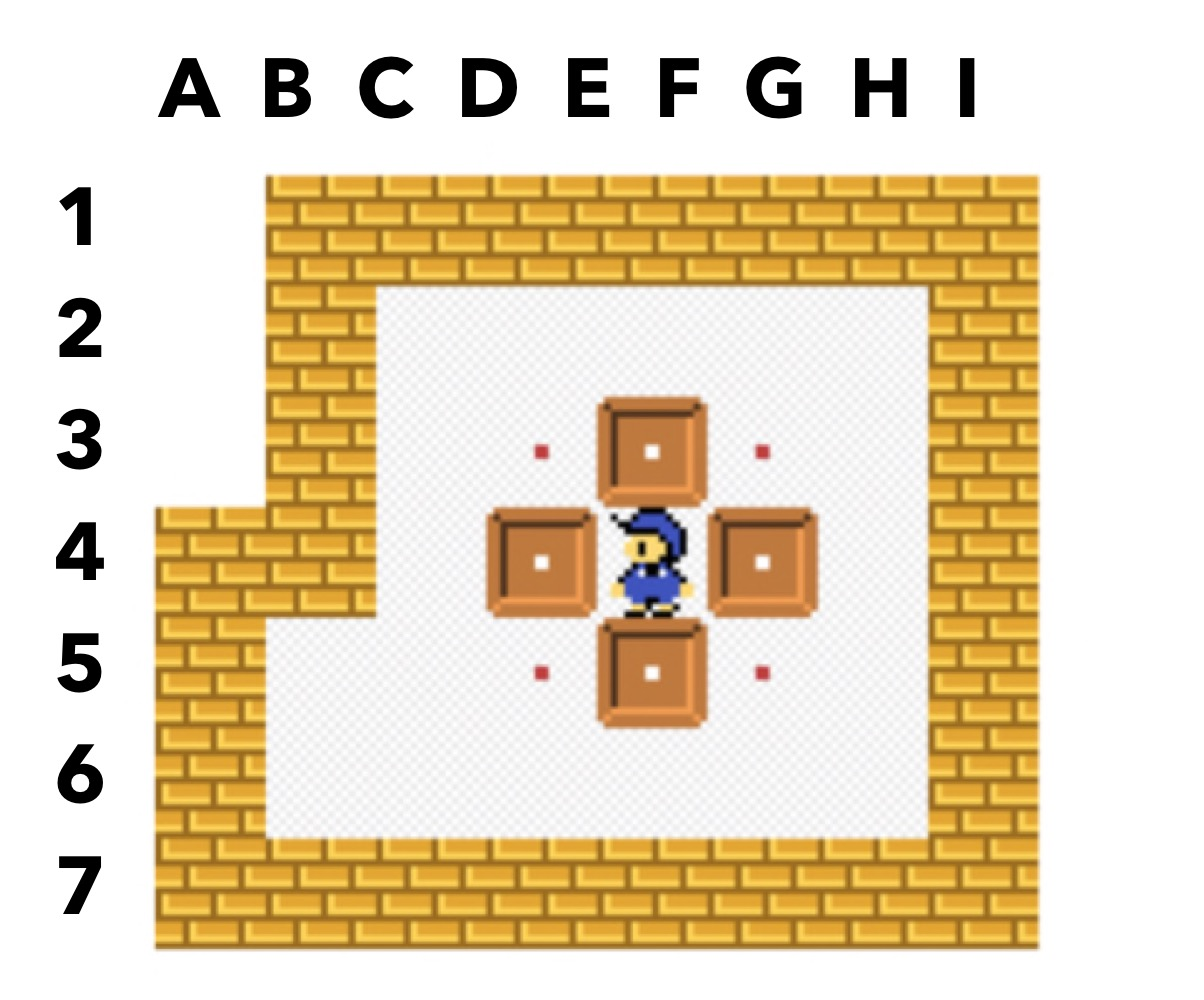
\includegraphics[width=2.8in]{figure1.JPG} \\
    \caption{Example of proposed Sokoban puzzle solved with 33 steps using OPTIC planner}\label{fig:example}
\end{figure}

\section{Part I: Designing a Planning Domain}
In the following section we will pick the most interesting parts of our domain and introduce reasoning behind designs and declarations in our domain.pddl file. 

\subsubsection{Domain constants}
To reinforce the idea of single-agent problem we have declared a player \emph{"p1"} as constant to avoid ambiguity of multi-players. Throughout our problem and domain file this player will be the only actor in our proposed world. 

\subsubsection{Domain predicates}
Probably the most important predicate from our domain is \texttt{(collected-box ?b -box)}. As being mentioned, the proposed domain file does restrict itself on specific goals (placing boxes on predefined squares). Instead our aim is to have all declared boxes \emph{"collected"} without explicitly mentioning where to position different boxes. We have in essence given a \emph{free-hand} and left the decision on the planner to find the \emph{"best-optimal solution"}. 

\subsubsection{Domain requirements}
Requirement declaration includes\texttt{ :constraints,:universal-preconditions, :typing,:fluents,:preferences }and\texttt{ :action-costs}. The reason behind declaration of above stated requirements is given as follows:

\begin{itemize}
\item \texttt{:typing} - reflect different object types in the domain i.e., player, box, square as single object declaration can’t represent all different entities in the domain.
\item \texttt{:universal-preconditions} - The use of universal quantifier spared us writing lengthy and tedious preconditions or goals. For instance, instead of listing all collected boxes (boxes on storage units) in conjunction in the form of \texttt{(:goal (and (collected-box \(b_1 ..b_n, b_n_+_1\))))} where \(n >= 1\) we could simply write \texttt{(:goal (forall (?b - box) (collected box)))} indicating that our \emph{hard goal} is to place all existing boxes on some storage units.
\item \texttt{:fluents} - We also exploit the feature of using complete numeric subset of PDDL and use numeric modelling throughout our domain file. Declaring numeric state variables through \texttt{:fluents} allowed numeric formulation of our actions i.e., break-noth-wall with precondition
\texttt{(>(bomb-available ?p) 0)} which restrict the occurrence of the action unless we have more than \(x >= 1\) bombs. Since Sokoban is PSPACE-complete problem, thus problem file evaluation can increase exponentially with size of the search space. For problem file simplification reasons, we have introduced pull action as oppose to traditional Sokoban game which only allows push . Expressed as pull-\emph{direction} with condition \texttt{(>(pliers-available) 0)} indicating that player is able to pull if it has the tool \emph{"plier"}. The number of pre-set pliers initialized in the ground function increases with difficulty of the problem file.  
\item \texttt{:preferences} - Declaration of preferences in the domain file enable us to achieve soft goals and define properties that we would like to achieve but are not compulsory. Thus, we have exploited this feature and defined that it will be preferable for the player to collect as much coins as possible. Implemented through \texttt{(:goal (preference (> (collected-coins) 0))}.
\item \texttt{:action-cost} -  For optimization reasons, every action in our action schema comes with  a cost which means that every move will incur penalty.  Our goal is to minimize incurred action cost in planning metric so minimum number of steps are taken to reach the objective.  This was realized through declaration of \texttt{:function (total-cost)},\texttt{:effect (increase (total-cost) 1)}and\texttt{ :metric (minimize (total-cost))}. 
\end{itemize}

\subsubsection{Domain actions}
The introduced action schema tries to mimic all possible moves taken by player. Every single action in the domain file is named in self-explanatory way i.e., pull-\emph{direction}, push-\emph{direction}, jump-\emph{direction}, break-\emph{direction} and pick-up-\emph{tool}(bomb, coin, trampoline). Implementing domain file using this kind of architecture allows better trackability of generated plan. It is also important to mentioned here that push and pull actions come in two different version i.e., push-\emph{direction}, push-\emph{direction}-to-hole. Former indicating a push to free location , latter indicating a push to hole or storage location (See following section for reason).

\subsubsection{Planner constraints and proposed solutions}
\textbf{OPTIC} planner provided lacks several important functionalities such as support for the \textbf{ADL}, conditional effects and negative preconditions. For such reasons we remodelled the action schema to avoid those features. As some action’s preconditions are made up of a single or clauses of \emph{k} terms, we have remodelled the problem to create \emph{k} copies of an action and used one term for each as a regular precondition i.e., instead of writing in the \texttt{:effect (when(hole-at ?box-after-move))} to represent condition when a box is moved on a hole after push or pull. We have re-written this into two push and pull actions i.e., push-up with \texttt{:precondition (no-hole-at ?box-after-move)} and push-up-to-hole with \texttt{:precondition (hole-at ?box-after-move)} and \texttt{:effect (collected-box ?box)}. As being mentioned \textbf{OPTIC}  also does not support negative precondition, therefore all predicates which needs to be negative in the precondition have been represented by two static predicates i.e., has- trampoline and has-no-trampoline to indicate that a player has this tool. While in principle this does allows \textbf{OPTIC} to work with this problem, but as a result it reduces efficiency and come at expense given increased number of actions required.   

\subsubsection{Possible domain improvements}
Although axioms do not increase language expressiveness, but it will be great to include \emph{derived predicates} as it decreases the domain description size and plan length, compiling away from axiom can result in an exponential growth in number of actions. In our case instead of listing all squares which are above one another in the problem file i.e., \texttt{(above sq-a1 sq-a2)} indicating square \emph{a1} being above \emph{a2}. We could have written \texttt{((: derived (above? a ?b - squares) (and (left-to b?  ?c) (above c? ?a))} that recursively defines relationship between pairs of squares.   


\end{document}
